\documentclass[a4paper, landscape, 10pt, twocolumn]{article}
\usepackage{xeCJK}
\usepackage[left=1.5cm, right=1.5cm, top=1.5cm, bottom=1.5cm]{geometry}
\usepackage{tabularx}
\usepackage{amsmath}
\usepackage{fancyhdr}
\usepackage[table]{xcolor}
\usepackage{ulem}
\usepackage{pgfplots}
\usepackage{adjustbox}
\usepackage{circuitikz}
\usepackage{paralist}
\raggedbottom
\pgfplotsset{compat=1.18}
\pgfplotsset{trig format plots=rad}
\usetikzlibrary{math, arrows.meta}
\pagestyle{fancy}
\lhead{高中物理}
\rhead{南昌学而思}
\cfoot{generated by Linghui Ding}
\setlength{\columnseprule}{0.4pt}
\begin{document}
\rowcolors{2}{white}{blue!10}
\renewcommand{\arraystretch}{1.5}
\noindent
\begin{tabularx}{\columnwidth}{XX}
  \rowcolor{blue!30}
  \multicolumn{2}{l}{\parbox[c][2.5\ht\strutbox][c]{0.9\columnwidth}{\Large 运动学}} \\
  \multicolumn{2}{l}{\textsf{运动学基本概念}}\\
  瞬时速度&$v=\lim_{t\to0} \frac{\Delta x}{\Delta t}$\\
  平均速度&$v=\frac{\Delta x}{\Delta t}$\\
  瞬时速率&$v=$瞬时速度大小\\
  平均速率&$v=\frac{\Delta s}{\Delta t}$\\
  平均加速度&$a=\frac{\Delta v}{\Delta t}$\\
  \multicolumn{2}{l}{\textsf{匀变速直线运动}}\\
  位移&$x=v_0t+\frac{1}{2}at^2$\\
  &$x=vt-\frac{1}{2}at^2$\\
  &$x=\frac12(v+v_0)t$\\
  速度&$v=v_0+at$\\
  速度平方&$v^2=v_0^2+2ax$\\
  中间位移速度&$v=\sqrt{\frac{x_1^2+x_2^2}2}$\\
  中间时刻速度&$v=\frac12(x_1+x_2)$\\
  第M段与第N段Ts时间内位移差&$(M-N)aT^2$\\
  \multicolumn{2}{l}{\textsf{从静止开始加速的规律}}\\
  相等时间每段位移比&$1:3:5:\cdots:2n-1$\\
  相等时间总计位移比&$1:4:9:\cdots:n^2$\\
  相等位移间隔每段用时比&$1:\sqrt2-1:\cdots:\sqrt n-\sqrt{n-1}$\\
  相等位移间隔总计用时比&$1:\sqrt2:\cdots:\sqrt n$\\
  \multicolumn{2}{l}{\textsf{自由落体}}\\
  自由落体高度&$h=\frac12gt^2$\\
  自由落体速度&$v=gt=\sqrt{2gh}$\\
\end{tabularx}
\newpage
\noindent{\large\textbf{注意}}\\
\textbf{刹车问题：}
凡是汽车这样的现实交通工具，认为刹车到0后不会掉头运动。\\而如果是抽象的物体，那么认为减速到0，
可以继续反向加速。\\利用$x=\frac{v^2}{2a}$求解位移是最稳妥的做法。\\
\textbf{反向多过程问题：}
\begin{center}
  \begin{tikzpicture}
    \coordinate (v1) at (0,0) {};
    \coordinate (v2) at (4,0) {};
    \coordinate (v3) at (4,2) {};
    \draw (v1) -- (v2) -- (v3) -- (v1);
    \coordinate (v4) at (3,1.5) {};
    \coordinate (v5) at (2.5,2.5) {};
    \coordinate (v6) at (1,0.5) {};
    \coordinate (v7) at (0.5,1.5) {};
    \draw (2,1) .. controls (6,3.5) and (-1,0) .. (0,0.5);
    \draw[dashed, red] (v4) -- (v5);
    \draw[dashed, red] (v6) -- (v7);
    \draw[blue,->] (2-0.25,1+0.5) -- (1-0.25,0.5+0.5) node [midway, left] {$-x$};
    \draw[black] (2-0.25,1+0.5) circle(0.5pt);
    \draw[red,->] (2-0.25,1+0.5) -- (3-0.25,1.5+0.5) node [midway, left] {$x$};
  \end{tikzpicture}
\end{center}
如图所示，一个斜面上物体做一个往返运动，最多会出现三个位移大小相等的点，最少出现两个位移
大小相等的点，最多两个速度大小相等的点，并且这两个点到出发点的位移相同。\\
\textbf{追及相遇：}
\begin{itemize}
  \item 大追小，最多相遇两次，速度相等时最近距离。
  \item 小追大，最多相遇一次，速度相等时最远距离。
\end{itemize}
相对速度与加速度求解相对位移公式：$\Delta x=\frac{(v_1-v_2)^2}{2|a_1-a_2|}$\\
利用相对位移公式可以快速解决两个匀变速直线运动的追及相遇问题。
\newpage
\noindent
\begin{tabularx}{\columnwidth}{XX}
  \rowcolor{blue!30}
  \multicolumn{2}{l}{\parbox[c][2.5\ht\strutbox][c]{0.9\columnwidth}{\Large 静力学}} \\
  重力&$G=mg$\\
  弹簧弹力&$F=k\Delta x$\\

  滑动摩擦力&$F=\mu N$\\
  合力范围&$|F_1-F_2|\le F \le |F_1+F_2|$\\
\end{tabularx}
\noindent{\large\textbf{注意}}\\
\textbf{绳模型：}
\begin{itemize}
  \item 轻绳，无质量，只能产生拉力。
  \item 有质量匀质绳，分析外力将绳看做质点，两侧张力方向为绳两端切线方向；分析内力时，
    取绳的一段作为研究对象，张力方向沿绳的切线方向，一段绳的质量使用占总体的比例计算，分
    析主要方法是隔离法。
\end{itemize}
\emph{活结}：绳子可以自由滑动，绳子的拉力在不同地方相等。\\
\emph{死结}：绳子固定，不同段的力的大小可以不相同。\\
\textbf{杆模型：}
\begin{itemize}
  \item 固定轻杆，可以提供任意方向的力，大小默认可以提供足够大的力。
  \item 铰链固定，此时杆失去了沿杆的移动能力，保留了绕铰链转动的能力。所以转动杆可以提供
    足够的沿杆的支持力或者拉力，但是垂直杆有一点点力就会转动，那么题目中要求的静止，也就意
    味着杆的垂直方向合力为0。
  \item 完全不固定的杆，比如一根杆子靠在墙上，此时杆子可以径向移动也可以绕轴转动，想要静
    止必须要垂直杆合力为0，沿杆的合力也为0才行。
\end{itemize}
\textbf{合力方向范围：}\\
合力的方向一定处于两个分力的夹角范围内，并且不会处于两个分力的所在直线上，除非某一个分力
大小为0。\\
\textbf{弹簧弹力：}\\
弹簧压缩时，弹力向两侧朝外，弹簧拉伸时，弹力指向内。弹簧弹力一定两侧相等，任何一侧的受力
一定是等于弹簧弹力。\\
并联弹簧劲度系数 $k_\text{并} = k_1 + k_2 + \cdots + k_n$\\
串联弹簧劲度系数 $\frac1{k_\text{串}} = \frac{1}{k_1} + \frac{1}{k_2} +
\cdots + \frac{1}{k_n}$\\
当只有两根弹簧时，串联和并联的关系可以简化为：
\[
  k_\text{并} = k_1 + k_2, \quad k_\text{串} = \frac{k_1 k_2}{k_1 + k_2}
\]
由此可以知道，把一根弹簧进行分割时，如果分成两段，分割后两段的劲度系数是原来的两倍！\\
分成$n$段，分割后每段的劲度系数是原来的$n$倍。\\
之后并联这些分段，整体的劲度系数达到了惊人的$n^2$倍！\\
\begin{itemize}
  \item
    \textbf{摩擦力的定义}：摩擦力是两个\emph{相互接触}并有\emph{相对运动趋势或相对运动}的物体之间，在接触面上产生的阻碍相对运动的力。\\
    摩擦力的方向总是与相对运动方向相反，或与相对运动趋势方向相反。
  \item \textbf{摩擦力的分类}：
    \begin{itemize}
      \item
        \emph{静摩擦力}：当物体间没有发生相对滑动，但有相对滑动趋势时，接触面之间产生的阻碍相对运动趋势的力叫静摩擦力。静摩擦力的大小随外力变化而变化，其最大值称为最大静摩擦力。
      \item \emph{滑动摩擦力}：当物体间发生相对滑动时，接触面之间产生的阻碍相对滑动的力叫滑动摩擦力。滑动摩擦力的大小通常为恒定值。
      \item \emph{滚动摩擦力}：当物体在另一物体表面滚动时，产生的阻碍滚动的力叫滚动摩擦力。滚动摩擦力远小于滑动摩擦力。
    \end{itemize}
  \item \textbf{摩擦力的产生条件}：
    \begin{itemize}
      \item 必须有两个物体相互接触，
      \item 相互产生弹力，
      \item 并且接触面具有粗糙性（微观不平），
      \item 且有相对运动或相对运动趋势。
    \end{itemize}
  \item \textbf{摩擦力的方向}：总是与物体相对运动方向或相对运动趋势方向相反。
  \item \textbf{摩擦力的计算公式}：
    \begin{itemize}
      \item 最大静摩擦力与正压力成正比，而静摩擦力本身与正压力无关。
      \item 滑动摩擦力：$f = \mu N$，其中$\mu$为滑动摩擦因数，$N$为正压力。
    \end{itemize}
  \item \textbf{摩擦因数}：摩擦因数与接触面的材料和粗糙程度有关，与接触面积大小无关。
  \item
    \textbf{静摩擦力的特点}：静摩擦力的大小不一定等于最大静摩擦力，而是根据实际需要“自适应”变化，直到达到最大静摩擦力为止。一旦外力超过最大静摩擦力，物体就会发生滑动，转为滑动摩擦力。
\end{itemize}
判断相对运动或相对运动趋势的方法有以下几种：
\begin{itemize}
  \item
    \textbf{速度法}：判断两个物体在接触面方向上的速度是否相同。如果速度不同，则存在相对运动；如果速度相同，则无相对运动，但需进一步判断是否有相对运动趋势。
  \item \textbf{受力分析法}：分析外力作用下，若没有摩擦力或摩擦力不足，物体是否会发生相对滑动。若会，则存在相对运动趋势。
  \item \textbf{极端假设法}：假设接触面光滑（无摩擦），判断物体是否会发生相对滑动。如果会，则存在相对运动趋势。
  \item \textbf{几何关系法}：通过分析物体的运动轨迹、转动或连接方式，判断接触面是否会产生相对滑动或滑动趋势。
\end{itemize}

\noindent 常用的判断顺序是：\\
先判断有无相对运动（速度是否相同），若无则判断有无相对运动趋势（极端假设法或受力分析法）。\\
\textbf{当出现超过两个力进行合成该如何处理？}\\
对任何两个力先进行合成，得到一个合力，然后再将这个合力与下一个力进行合成，依次类推，直到所有力都被合成。\\
\textbf{当需要分解为超过两个力该如何处理？}\\
对一个力进行分解时，可以选择任意两个方向进行分解，得到两个分力。然后可以将其中一个分力继续分解为两个方向的分力，依次类推，直到分解为所需的分力数量。\\
\textbf{多个力合成时大小范围如何确定？}\\
任意两个力先求出范围$[|F_1 - F_2|, F_1 + F_2]$。\\
接着第三个力与这个范围进行合成，需要注意最小值。举几个例子：\\
三个力大小分别是4、4、6，那么首先得到$[0,8]$，接着得到[0,14]，其实就是力的大小范围不能是负数，而且6在范围内，所以可以得到最小的0.\\
如果是4、4、10，那么首先得到$[0,8]$，接着，你会注意到我们无法获得0这个最小值，范围是$[2,18]$。\\
如果是4、8、3，首先得到$4,12$，接着无法得到0，只能找最小值，于是有范围$1,15$\\
上面的范围计算，虽然我们选取的顺序是特定的，但是结论是通用的，你不管怎么调整顺序不会影响结论。\\
\textbf{受力分析怎么做？}\\
重力先画，不一定要画在重心位置，或者是中心点。\\
挑一个好看的地点更好，比如图中已经有很多直线了，选择那些直线的交点，这样可以让图像更清晰。\\
弹力是一个难点，牢记我们之前的规律应用他们，\\
最后再画摩擦力，因为有弹力才能有摩擦力。\\
总结为1重2弹3摩擦。最后题目中还有别的外力再补充。\\
二力平衡，一定是等大反向，作用于同一个物体，方向是一条直线上。\\
不共线的三力平衡一定是形成一个首尾相连的密闭三角形。\\
多个力作用平衡时，任意一个力与其他力的合力是二力平衡。\\
在上面的过程中，唯一需要注意的就是，多个力的合力不要和其他任何一个分力同时存在，一旦选择了合成，那么这些力就应该消失。\\
正交分解处理平衡问题，只需要在两个垂直的方向上，合力为0就是平衡。一个方向平衡，那么就是那个方向上合力为0.\\
三个力及以下，我们很少使用正交分解方法，最多使用正弦定理。四个力则基本上都要用正交分解解决。\\
\textbf{正交分解求解共点力平衡：}\\
共点力平衡问题常用正交分解法。将所有力分解到两个互相垂直的方向（如水平和竖直，或沿斜面和垂直斜面），分别列出每个方向上的分力代数和为零的方程：
\[
  \sum F_x = 0,\quad \sum F_y = 0
\]
这样可以将力的平衡问题转化为两个独立的代数方程，便于求解未知力的大小和方向。\\
\textbf{三个力的动态平衡问题：}\\
\textbf{情形一：重力恒定，另一个力方向恒定，第三力变化}\\
设$G$为重力，$F_1$方向恒定，$F_2$大小可以发现变化过程为先变小后变大，如果$F_1$的与重力的夹角是$90^\circ$那么，只有变小过程。\\
\textbf{情形二：重力恒定，另一个力大小恒定，第三力变化}\\
设$G$为重力，$F_1$大小恒定，则利用余弦定理知道，当两个力的大小不变的时候，随着$F_1$与重力的夹角从小变大的过程，$F_2$在逐渐增大。\\
% 动态三角形法则示意图
\begin{minipage}{0.48\columnwidth}
  \centering
  \textbf{情形一：重力和$F_1$方向不变}\\
  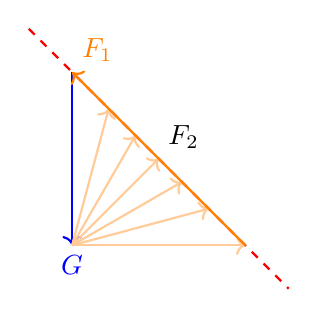
\begin{tikzpicture}[scale=1.1]
    % 重力
    \draw[->,thick,blue] (0,0) -- (0,-2) node[below] {$G$};
    % F1方向恒定
    \draw[thick,red,dashed] (-0.5,0.5) -- (2.5,-2.5);
    % F2动态过程（用淡色虚线表示运动轨迹）
    \foreach \a in {0,15,...,75} {
      \draw[->,orange!40!white,thick] (0,-2) -- ++
      ({2/(1+tan(\a))},{2*tan(\a)/(1+tan(\a))});
    }
    \draw (1,-1) node [ above right ] {$F_2$};
    \draw[->,thick,orange] (2,-2) -- (0,0) node[above right] {$F_1$};
  \end{tikzpicture}
\end{minipage}
\hfill
\begin{minipage}{0.48\columnwidth}
  \centering
  \textbf{情形二：重力和$F_1$大小不变}\\
  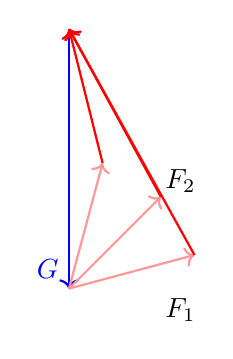
\begin{tikzpicture}[scale=1.1]
    % 重力
    \draw[->,thick,blue] (0,3) -- (0,0) node[above left] {$G$};
    % F1大小恒定，方向变化（用淡色虚线表示运动轨迹）
    \foreach \a in {15,45,75} {
      \draw[->,red!40!white,thick] (0,0) -- ({1.5*cos(\a)}, {1.5*sin(\a)});
      \draw[->,thick,red] ({1.5*cos(\a)}, {1.5*sin(\a)}) -- (0,3);
    }
    \draw (1,0) node [ below right ] {$F_1$};
    \draw (1,1) node [ above right ] {$F_2$};
  \end{tikzpicture}
\end{minipage}
上面的图怎么用？要根据物体的实际移动情况得出力的方向变化情况，再根据某个已知力的方向变化情况得出
其他未知力的方向和大小变化情况。
\newpage
\noindent
\begin{tabularx}{\columnwidth}{XX}
  \rowcolor{blue!30}
  \multicolumn{2}{l}{\parbox[c][2.5\ht\strutbox][c]{0.9\columnwidth}{\Large 动力学}} \\
  牛顿第二定律&$F=ma$\\
\end{tabularx}
\noindent{\large\textbf{注意}}\\
牛二公式中的加速度是瞬时加速度。\\
这才是加速度的定义式，能够决定任意时刻的加速度，\\
并且只要物体的力改变了，物体的加速度就会改变。\\
静力平衡是加速度为零的情况。\\
对于之前我们的正交分解多了一种分解方法，沿加速度和垂直加速度分解，这样就不用分解加速度。\\
垂直方向的力之间互不影响，有着各自的牛顿运动定律表达式。\newline
\begin{minipage}{0.8\columnwidth}
  \centering
  \textbf{斜面上小球受力分析}\\
  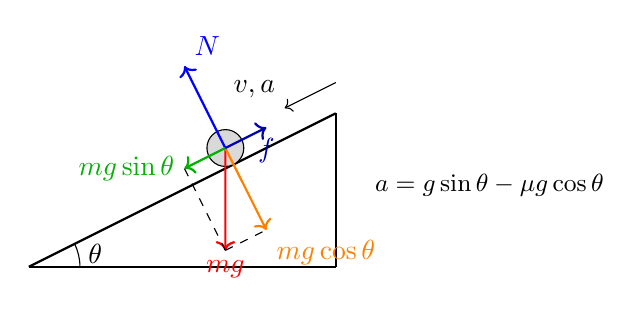
\begin{tikzpicture}[scale=1.3]
    % 斜面
    \draw[thick] (0,0) -- (3,0);
    \draw[thick] (0,0) -- (3,1.5);
    \draw[thick] (3,0) -- (3,1.5);
    \coordinate (O) at (2-0.08, 1+0.16);
    \coordinate (A) at ($(O) + (-0.4,-0.2)$);
    \coordinate (B) at ($(O) + (0.4,-0.8)$);
    \coordinate (G) at ($(O) + (0,-1)$);
    \coordinate (F) at ($(O) + (0.4,0.2)$);

    % 小球
    \filldraw[fill=gray!30] (O) circle (0.18);
    % 重力
    \draw[->,thick,red] (O) -- (G) node[below] {$mg$};
    % 支持力
    \draw[->,thick,blue] (O) -- ++(-0.4,0.8) node[above right] {$N$};
    % 分解分力
    \draw[->,thick,orange] (O) -- (B) node[below right] {$mg\cos\theta$};
    \draw[->,thick,green!70!black] (O) -- (A) node[left] {$mg\sin\theta$};

    \draw[->,thick,blue!70!black] (O) -- (F) node[below] {$f$};

    \draw[dashed] (G) -- (A);
    \draw[dashed] (G) -- (B);

    \draw[->] (3,1.8) -- (2.5, 1.55) node[above left] {$v,a$};
    % 斜面角度
    \draw (0.5,0) arc (0:26.565:0.5);
    \node at (0.65,0.13) {$\theta$};
    % 加速度表达式
    \node[below] at (4.5,1) {\small $a = g\sin\theta-\mu g\cos\theta$};
  \end{tikzpicture}
\end{minipage}\\
\textbf{超重、失重：}
有向上加速度，就是超重，此时合力向上，那么支持力会大于重力。有向下加速度就是失重，向下的
加速度为$g$，那就是完全失重。此时支持力小于重力。\\
任何蹲下、起立这种从静止运动最后静止的运动都会有一个超重过程也还有一个失重过程。\\
蹲下时，先失重后超重；起立时，先超重后失重。\\
\textbf{牛顿第一运动定律（惯性定律）}
质量是惯性的量度，质量越大惯性就越大。\\
惯性是物体改变运动状态难易程度的体现。\\
为什么我们之前质点，保留了质量呢？就是因为质量会影响惯性，而惯性会影响物体运动状态改变。所以运动学问题需要质量。\\
\textbf{惯性参考系是什么？}\\
将相对于地面这样的参考系，静止或者做匀速直线运动的参考系称为惯性参考系，简称惯性系。\\
在惯性系中牛二是成立的。\\

\begin{minipage}{0.48\columnwidth}
  \centering
  \textbf{惯性系（地面做参考系）}\\
  \begin{tikzpicture}[scale=1.1]
    % 电梯框
    \draw[thick] (0,0) rectangle (2,3);
    % 电梯加速度箭头
    \draw[->,thick,orange] (2.2,2.5) -- ++(0,-0.8) node[right] {$a$};
    % 物体
    \filldraw[fill=gray!30] (0.7,0.3) rectangle (1.3,0.8);
    % 物体受力箭头
    \draw[->,thick,blue] (1,0.8) -- ++(0,0.7) node[right] {$N$};
    \draw[->,thick,red] (1,0.3) -- ++(0,-0.7) node[right] {$mg$};
    % 公式
    \node[align=left] at (1,-1.0) {\small $mg-N=ma$};
    % 说明
    \node[align=left] at (1,3.3) {\small 认为电梯加速下落\\（惯性系角度思考）};
  \end{tikzpicture}
\end{minipage}
\hfill
\begin{minipage}{0.48\columnwidth}
  \centering
  \textbf{非惯性系（以电梯为参考系）}\\
  \begin{tikzpicture}[scale=1.1]
    % 电梯框
    \draw[thick] (0,0) rectangle (2,3);
    % 电梯加速度箭头
    \draw[->,thick,orange!60!white] (2.2,2.5) -- ++(0,-0.8) node[right] {$a$};
    % 物体
    \filldraw[fill=gray!30] (0.7,0.3) rectangle (1.3,0.8);
    % 物体受力箭头
    \draw[->,thick,blue] (1,0.8) -- ++(0,0.7) node[right] {$N$};
    \draw[->,thick,red] (1,0.3) -- ++(0,-0.7) node[right] {$mg$};
    \draw[->,thick,green] (1,1.5) -- ++(0,0.7) node[left] {$ma$,非惯性力};
    % 公式
    \node[align=left] at (1,-1.0) {\small $mg-N-ma = m \cdot
    0$\\\small (此时$a=0$)这符合认为物体静止假设。};
    % 说明
    \node[align=left] at (1,3.3) {\small 认为电梯静止或匀速\\（非惯性系角度思考）};
  \end{tikzpicture}
\end{minipage}
\textbf{有非惯性参考系吗？}\\
所有相对于地面这样的参考系，有着不等于0的加速度的参考系都是非惯性参考系，简称非惯性系。\\
在非惯性系中，牛顿运动定律不再适用，需要引入虚拟力来分析物体的运动。\\
这个虚拟力叫做非惯性力，大小等于物体的质量乘以参考系的加速度，方向与参考系的加速度方向相反。\\
\textbf{为什么会使用非惯性力？}\\
使用非惯性力可以把包含加速度的运动转换成静态平衡，这就使得我们可以使用该方法把所有的力学
问题转换成静态平衡去做。一套方法解决两种题目。\\
而且使用非惯性力更符合初学者的思考方式，这个时候不用去考虑合力方向，分力方向，只有一种
分析模式，就是合力为0。\\
\end{document}
